\chapter{Background}
To better understand this thesis work, a brief excursus of the existing literature about the main concepts the project relies on is presented. The aim is to provide some basic knowledge of the topics to understand what is considered state-of-the-art and to introduce some of the technologies exploited to develop the project.

\section{Multi-Agent Systems}
\subsection{What is an Agent?}
The concept of a software agent can be traced back to the early days of research into Distributed AI in the 1970s when Carl Hewitt proposed the concurrent Actor model.
In his paper, he introduced the concept of a self-contained, interactive, and concurrently-executing object which he termed ``actor''.
The latter is a computational agent with a mail address and behavior. Actors can communicate by message-passing and carry out their actions concurrently.~\cite{hewitt1977viewing}

The term ``agent'' quickly spread to heterogeneous research fields; therefore, there is no commonly agreed definition for it.
However, a generally accepted description of what an agent is is the following by Wooldridge~\cite{490039}:
\begin{quote}
    \textit{An agent is a self-contained program capable of controlling its own decision-making and acting, based on its perception of its environment, in pursuit of one or more objectives.}
\end{quote}
To sum up, we can identify a set of features that an agent should possess:
\begin{itemize}
    \item \textbf{Autonomy}: agents should be able to perform most of their tasks without the direct intervention of humans or other agents, and they should encapsulate control over their actions and internal state
    \item \textbf{Social ability}: agents should be able to interact with each other and possibly humans to complete their tasks.
    \item \textbf{Responsiveness} (situatedness): agents should perceive their environment and respond to changes in it.
    \item \textbf{Proactiveness}: agents should exhibit opportunistic, goal-directed behavior and take the initiative when appropriate.
\end{itemize}

During the first years, the research concentrated on interaction and communication among agents, decomposition and distribution of tasks, and coordination and cooperation.
The goal was to specify, analyze, design, and integrate systems containing multiple collaborative agents.

\subsection{From the Individual to the Collective}
Multi-Agent Systems have been studied as a per se field since the 1980s and gained widespread recognition in the 1990s.
Since then, international interest in the topic has grown enormously as agents are considered an appropriate paradigm to exploit the possibilities presented by massive open distributed systems.
Moreover, MAS seem to be a natural metaphor for understanding and building a wide range of what we might call \textit{artificial social systems}.~\cite{wooldridge2009introduction}

According to the \textit{Alan Turing Institute}~\cite{turing}
\begin{quote}
    \textit{A Multi-Agent System consists of multiple decision-making agents which interact in a shared environment to achieve common or conflicting goals.}
\end{quote}

\begin{figure}
    \centering
    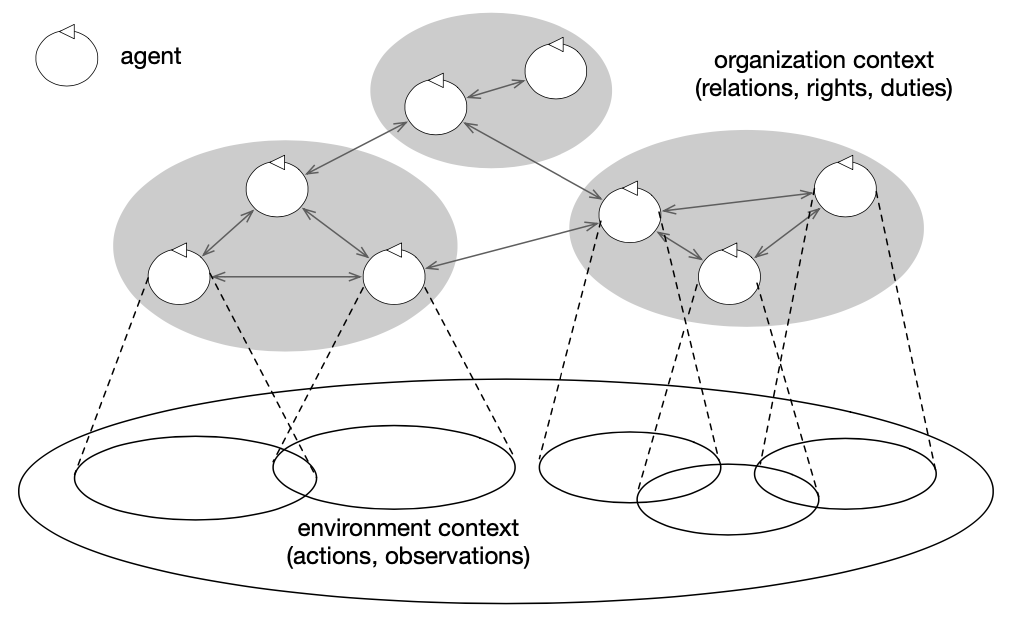
\includegraphics[width=0.9\linewidth]{images/multi-agent-systems.png}
    \caption{A representation of Multi-Agent Systems.~\cite{jennings2000agent}}
    \label{fig:multi-agent-systems}
\end{figure}
As it can be noticed in \cref{fig:multi-agent-systems}, MAS are composed of an environment and agents existing within it that are bonded by relations.

\subsubsection{Environment}
The environment in MAS plays a dual role~\cite{weyns2007environment}:
\begin{itemize}
    \item \textit{The ``external world''}.
    Agents become aware of the context they are immersed in and its dynamics by perceiving the environment through sensors.
    Moreover, they pursue their goals through actions performed by actuators that aim at modifying the environment, eventually reaching the latter's desired state.
    \item \textit{A medium for coordination}.
    Agents exploit the environment to share information and coordinate their behavior.
    Each agent follows simple behavioral rules, resulting in a collective behavior that is more complex than the sum of the individual behavior; this pattern resembles stigmergic systems in which agents coordinate their behavior through the manipulation of marks.
\end{itemize}
The environment not only enables the agents to interact with the deployment context, giving them access to sensors and actuators but also provides them with external resources that they can exploit to achieve their goal.

The \textit{Agents \& Artifacts} (A\&A) conceptual framework~\cite{ricci2007artifacts} argues that, just like in human society, MAS environments should contain different kinds of objects, tools, and artifacts in general that agents can use to support their activities.
This vision also constitutes a revolution from an engineering perspective as it encourages system designers to model the environment as a set of \textit{artifacts}, each of which encapsulates its intended purpose and exposes its observable state.
Moreover, the A\&A meta-model provides an effective abstraction level that shields low-level details of the deployment context, so that designers can focus on the agents' behavior.

\subsubsection{Organization}
There are two approaches to MAS engineering.~\cite{Ahmed_Abbas_2015}
The first one regards \textit{agent-centered} MAS, in which the focus is given to individual agents.
According to this viewpoint, the designer should concern about the local behavior of the agents and their interactions without worrying about the global structure and goal of the system as the latter should emerge as a result of the lower-level individual interactions in a bottom-up fashion.
The key issues of this approach are unpredictability and uncertainty since it could lead to undesirable emergent behaviors.
As Weyns~\cite{weyns2010organizations} stated, giving the responsibility of system organization implicitly to individual agents is highly complex and not suitable for real-world large-scale scenarios.

The second approach is \textit{organization-centered} MAS, in which the structure of the system is given greater attention.
The developer designs the entire organization and coordination patterns on the one hand, and the agents' local behavior on the other.
This can be seen as a top-down approach as the organization abstractions impose constraints on the agents and regulate their interactions, simplifying the design of complex and scalable systems and allowing more accurate modeling of the problems being tackled.

\section{Organizations in Multi-Agent Systems}
\subsection{Organizational Models}
\subsection{The MOISE+ Model}

\section{Hypermedia Multi-Agent Systems}
